\documentclass[unknownkeysallowed]{beamer}
\usepackage[french,english]{babel}
\usepackage{./tex/sty/beamer_js}
\usepackage{./tex/sty/shortcuts_js}
\usepackage{etex}
\usepackage{csquotes}
\usepackage{stmaryrd}


\addbibresource{bibli.bib}



\begin{document}


%%%%%%%%%%%%%%%%%%%%%%%%%%%%%%%%%%%%%%%%%%%%%%%%%%%%%%%%%%%%%%%%%%%%%%%%%%%%%%%
%%%%%%%%%%%%%%%%%%%%%%             Headers               %%%%%%%%%%%%%%%%%%%%%%
%%%%%%%%%%%%%%%%%%%%%%%%%%%%%%%%%%%%%%%%%%%%%%%%%%%%%%%%%%%%%%%%%%%%%%%%%%%%%%%



%%%%%%%%%%%%%%%%%%%%%%%%%%%%%%%%%%%%%%%%%%%%%%%%%%%%%%%%%%%%%%%%%%%%%%%%%%%%%%%
\begin{frame}
\bigskip
\bigskip
\begin{center}{
\LARGE\color{marron}
\textbf{HMMA308 - Project}
\textbf{ }\\
\vspace{0.5cm}
}

\color{marron}
\textbf{Recommendation system}
\end{center}

\vspace{0.5cm}

\begin{center}
\textbf{Fanchon Herman} \\
\vspace{0.1cm}
\url{https://github.com/fanchonherman/HMMA308-Project}\\
\vspace{0.5cm}
University of Montpellier \\
\end{center}

\centering

\includegraphics[width=0.13\textwidth]{./images/Logo}

\end{frame}
%%%%%%%%%%%%%%%%%%%%%%%%%%%%%%%%%%%%%%%%%%%%%%%%%%%%%%%%%%%%%%%%%%%%%%%%%%%%%%%


%%%%%%%%%%%%%%%%%%%%%%%%%%%%%%%%%%%%%%%%%%%%%%%%%%%%%%%%%%%%%%%%%%%%%%%%%%%%%%%
%%%%%%%%%%%%%%%%%%%%%%%%       PLAN      %%%%%%%%%%%%%%%%%%%%%%%%%%%%%%%%%%%%%%
%%%%%%%%%%%%%%%%%%%%%%%%%%%%%%%%%%%%%%%%%%%%%%%%%%%%%%%%%%%%%%%%%%%%%%%%%%%%%%%



%%%%%%%%%%%%%%%%%%%%%%%%%%%%%%%%%%%%%%%%%%%%%%%%%%%%%%%%%%%%%%%%%%%%%%%%%%%%%%%
\begin{frame}{Table of Contents}
\tableofcontents
\end{frame}
%%%%%%%%%%%%%%%%%%%%%%%%%%%%%%%%%%%%%%%%%%%%%%%%%%%%%%%%%%%%%%%%%%%%%%%%%%%%%%%

%%%%%%%%%%%%%%%%%%%%%%%%%%%%%%%%%%%%%%%%%%%%%%%%%%%%%%%%%%%%%%%%%%%%%%%%%%%%%%%
\AtBeginSection[]
{
\begin{frame}<beamer>{Table of Contents}
\tableofcontents[currentsubsection,
    hideothersubsections,
    sectionstyle=show/shaded,
]
\end{frame}
}
%%%%%%%%%%%%%%%%%%%%%%%%%%%%%%%%%%%%%%%%%%%%%%%%%%%%%%%%%%%%%%%%%%%%%%%%%%%%%%%


%%%%%%%%%%%%%%%%%%%%%%%%%%%%%%%%%%%%%%%%%%%%%%%%%%%%%%%%%%%%%%%%%%%%%%%%%%%%%%%
%%%%%%%%%%%%%%%%%%%%%%%%%%%%%%%%%%%%%%%%%%%%%%%%%%%%%%%%%%%%%%%%%%%%%%%%%%%%%%%
\section{Introduction}
\label{sec:introdcution}
%%%%%%%%%%%%%%%%%%%%%%%%%%%%%%%%%%%%%%%%%%%%%%%%%%%%%%%%%%%%%%%%%%%%%%%%%%%%%%
%%%%%%%%%%%%%%%%%%%%%%%%%%%%%%%%%%%%%%%%%%%%%%%%%%%%%%%%%%%%%%%%%%%%%%%%%%%%%%%

%%%%%%%%%%%%%%%%%%%%%%%%%%%%%%%%%%%%%%%%%%%%%%%%%%%%%%%%%%%%%%%%%%%%%%%%%%%%%%%
\begin{frame}{Introduction}
\begin{itemize}
    \item Predict ratings that a user will give to a film that he doesn't know, 
    \item matrix factorization, 
    \item MovieLens 100k.
\end{itemize}
\end{frame}
%%%%%%%%%%%%%%%%%%%%%%%%%%%%%%%%%%%%%%%%%%%%%%%%%%%%%%%%%%%%%%%%%%%%%%%%%%%%%%%

%%%%%%%%%%%%%%%%%%%%%%%%%%%%%%%%%%%%%%%%%%%%%%%%%%%%%%%%%%%%%%%%%%%%%%%%%%%%%%%
%%%%%%%%%%%%%%%%%%%%%%%%%%%%%%%%%%%%%%%%%%%%%%%%%%%%%%%%%%%%%%%%%%%%%%%%%%%%%%%
\section{Data presentation}
\label{sec:data}
%%%%%%%%%%%%%%%%%%%%%%%%%%%%%%%%%%%%%%%%%%%%%%%%%%%%%%%%%%%%%%%%%%%%%%%%%%%%%%
%%%%%%%%%%%%%%%%%%%%%%%%%%%%%%%%%%%%%%%%%%%%%%%%%%%%%%%%%%%%%%%%%%%%%%%%%%%%%%%

%%%%%%%%%%%%%%%%%%%%%%%%%%%%%%%%%%%%%%%%%%%%%%%%%%%%%%%%%%%%%%%%%%%%%%%%%%%%%%%
\begin{frame}{Data presentation}
\begin{itemize}
    \item $100,000$ ratings,
    \item $943$ users,
    \item $1682$ movies,
    \item each user rated at least $20$ movies,
\end{itemize}
\begin{center}
    \begin{tabular}{|c|c|c|c|c|c|}
    \hline
         & user ID & movie ID & rating & timestamp \\
         \hline \hline
         0 & 196 & 242 & 3 & 881250949\\
         1 & 186 & 302 & 3 & 891717742\\
         2 & 22 & 377 & 1 & 878887116\\
         \hline
    \end{tabular}
    \captionof{table}{Extraction of some data.} 
\end{center}
\begin{itemize}
    \item convert the timestamp column.
\end{itemize}
\end{frame}
%%%%%%%%%%%%%%%%%%%%%%%%%%%%%%%%%%%%%%%%%%%%%%%%%%%%%%%%%%%%%%%%%%%%%%%%%%%%%%%

%%%%%%%%%%%%%%%%%%%%%%%%%%%%%%%%%%%%%%%%%%%%%%%%%%%%%%%%%%%%%%%%%%%%%%%%%%%%%%%
\begin{frame}[plain]{}
    \begin{center}
        \color{marron}
        \LARGE Visualizations of some data
    \end{center}
\end{frame}
%%%%%%%%%%%%%%%%%%%%%%%%%%%%%%%%%%%%%%%%%%%%%%%%%%%%%%%%%%%%%%%%%%%%%%%%%%%%%%%

%%%%%%%%%%%%%%%%%%%%%%%%%%%%%%%%%%%%%%%%%%%%%%%%%%%%%%%%%%%%%%%%%%%%%%%%%%%%%%%
\addtocounter{framenumber}{-1}
\begin{frame}{Visualizations}
  \begin{figure}[H]
\centering
\begin{subfigure}{.5\textwidth}
  \centering
  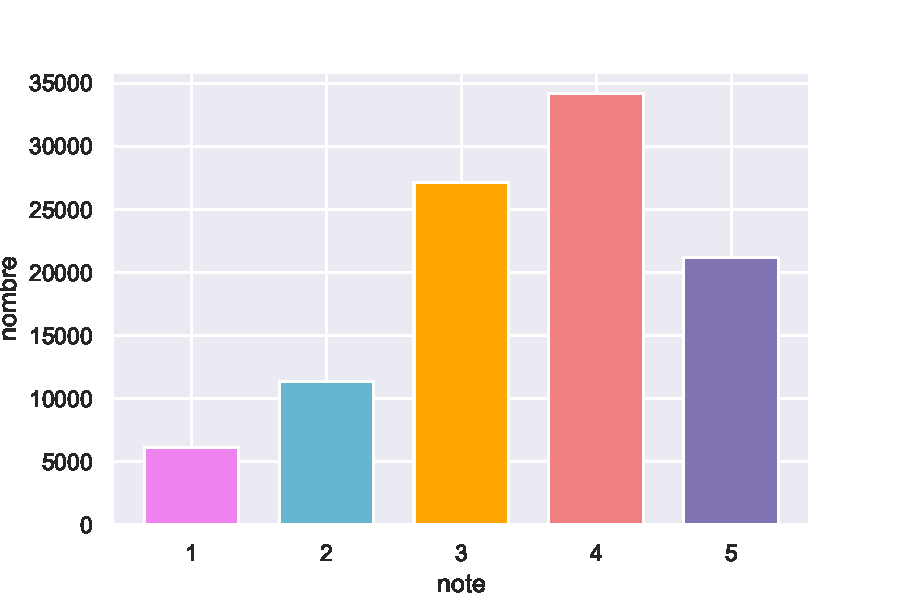
\includegraphics[width=1\linewidth]{./images/distrib_notes.pdf}
  \caption{Ratings distributions.}
  \label{fig:distri_notes}
\end{subfigure}%
\begin{subfigure}{.5\textwidth}
  \centering
  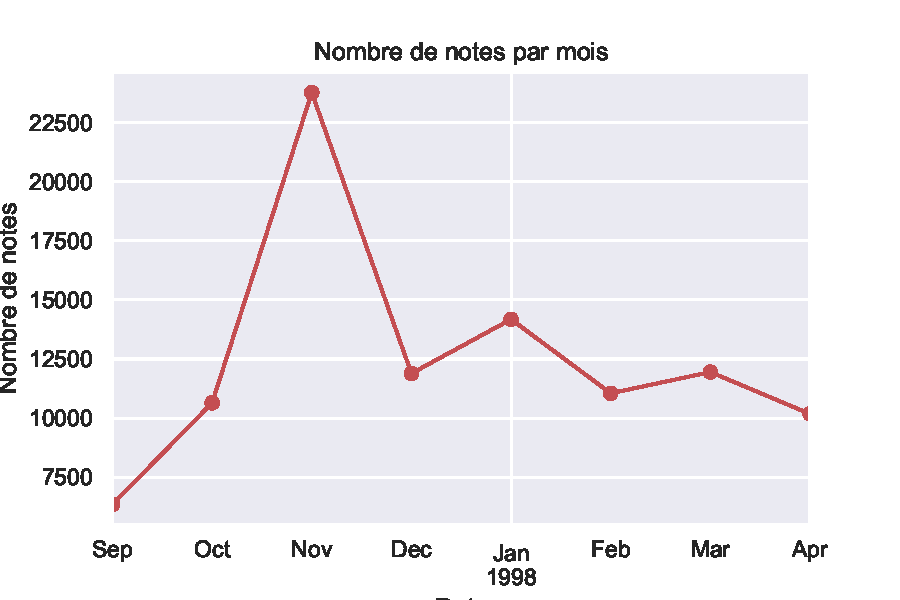
\includegraphics[width=1\linewidth, clip,trim={0cm 0cm 0cm 0.6cm} ]{./images/notes_mois.pdf}
  \caption{Number of ratings per month.}
  \label{fig:resid_}
\end{subfigure}
\caption{Graphical representation of data.}
\label{fig:notes_mois}
\end{figure}  
\end{frame}
%%%%%%%%%%%%%%%%%%%%%%%%%%%%%%%%%%%%%%%%%%%%%%%%%%%%%%%%%%%%%%%%%%%%%%%%%%%%%%%

%%%%%%%%%%%%%%%%%%%%%%%%%%%%%%%%%%%%%%%%%%%%%%%%%%%%%%%%%%%%%%%%%%%%%%%%%%%%%%%
\begin{frame}{Visualizations}
    \begin{figure}[H]
\centering
  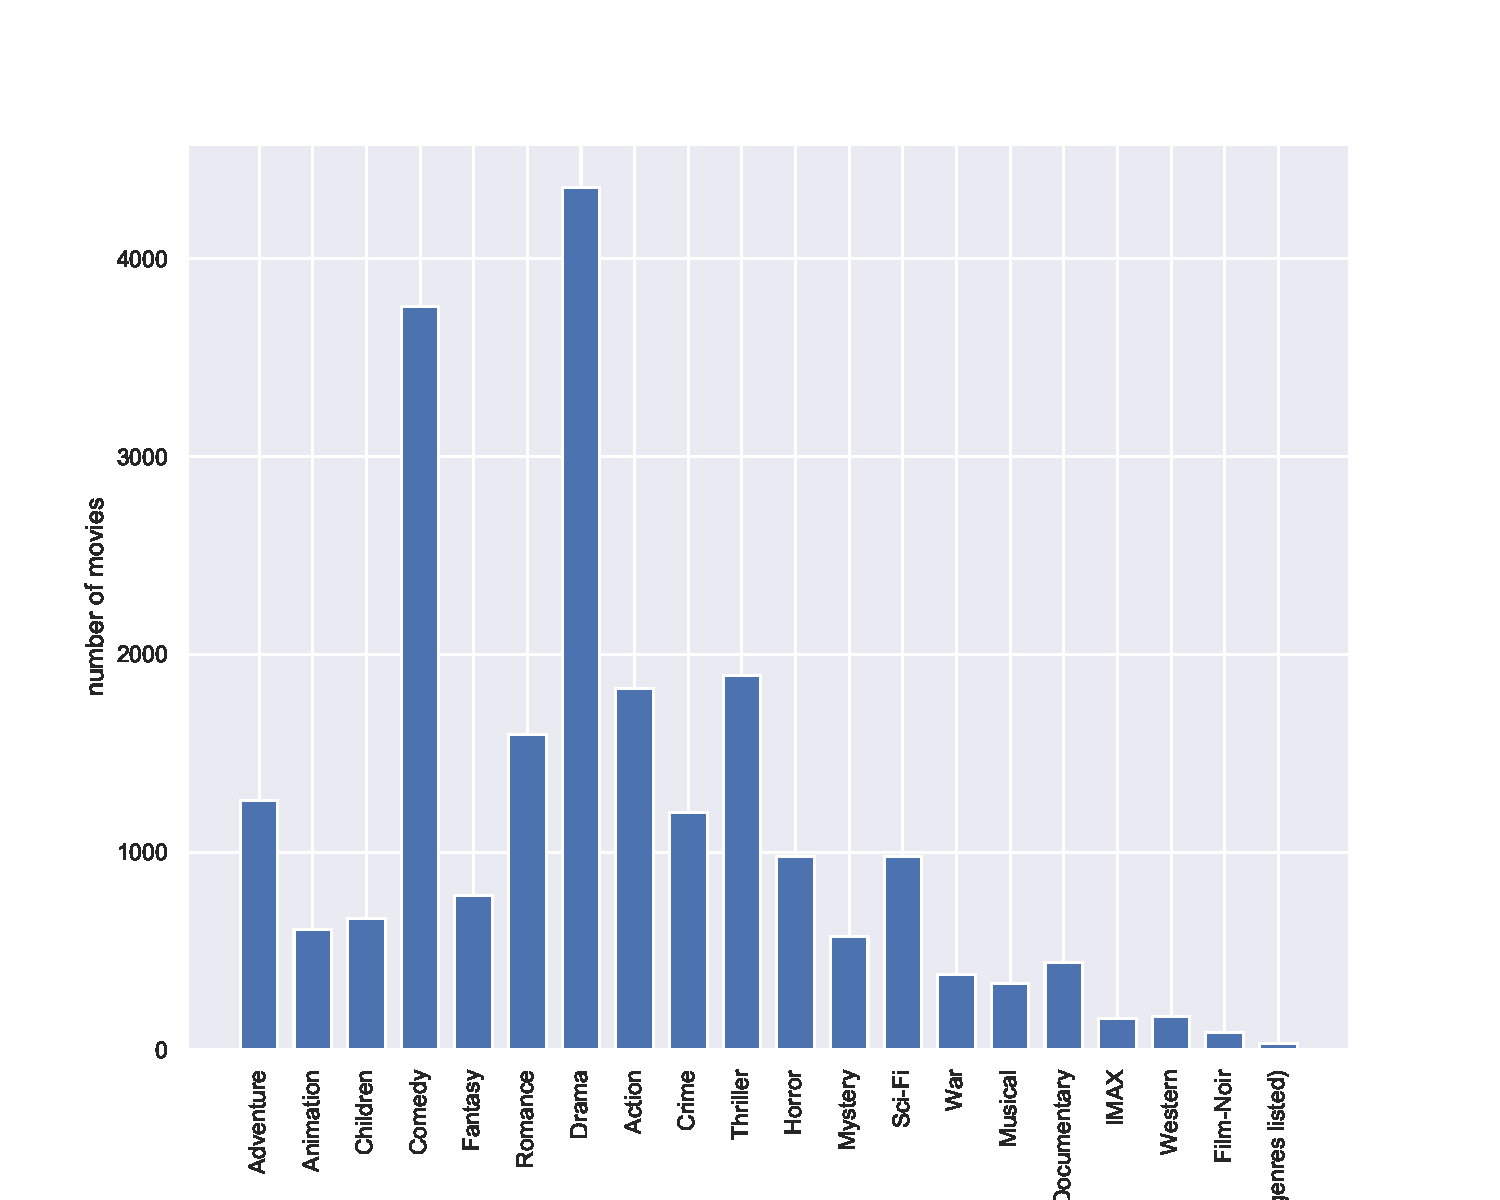
\includegraphics[scale=0.35]{./images/genres.pdf}
  \caption{Number of movies per category.}
  \label{fig:category}
\end{figure}
\end{frame}
%%%%%%%%%%%%%%%%%%%%%%%%%%%%%%%%%%%%%%%%%%%%%%%%%%%%%%%%%%%%%%%%%%%%%%%%%%%%%%%


%%%%%%%%%%%%%%%%%%%%%%%%%%%%%%%%%%%%%%%%%%%%%%%%%%%%%%%%%%%%%%%%%%%%%%%%%%%%%%%
%%%%%%%%%%%%%%%%%%%%%%%%%%%%%%%%%%%%%%%%%%%%%%%%%%%%%%%%%%%%%%%%%%%%%%%%%%%%%%%
\section{Matrix factorisation}
\label{sec:matrix}
%%%%%%%%%%%%%%%%%%%%%%%%%%%%%%%%%%%%%%%%%%%%%%%%%%%%%%%%%%%%%%%%%%%%%%%%%%%%%%
%%%%%%%%%%%%%%%%%%%%%%%%%%%%%%%%%%%%%%%%%%%%%%%%%%%%%%%%%%%%%%%%%%%%%%%%%%%%%%%

%%%%%%%%%%%%%%%%%%%%%%%%%%%%%%%%%%%%%%%%%%%%%%%%%%%%%%%%%%%%%%%%%%%%%%%%%%%%%%%
\subsection{Sparse matrix}
\label{sec:sparse}
%%%%%%%%%%%%%%%%%%%%%%%%%%%%%%%%%%%%%%%%%%%%%%%%%%%%%%%%%%%%%%%%%%%%%%%%%%%%%%%

%%%%%%%%%%%%%%%%%%%%%%%%%%%%%%%%%%%%%%%%%%%%%%%%%%%%%%%%%%%%%%%%%%%%%%%%%%%%%%%
\begin{frame}{Sparse matrix}
\begin{onlyenv}<1>
    $$Y=\begin{bmatrix}
5 & 3 & 4 & \dots & 0 & 0 & 0\\
4 & 0 & 0 & \dots & 0 & 0 & 0\\
0 & 0 & 0 & \dots & 0 & 0 & 0\\
  &   &   & \vdots\\
5 & 0 & 0 & \dots & 0 & 0 & 0\\
0 & 0 & 0 & \dots & 0 & 0 & 0\\
0 & 5 & 0 & \dots & 0 & 0 & 0\\
\end{bmatrix} \in \bbR^{n \times p}$$
\end{onlyenv}
\begin{onlyenv}<2->
    $$Y=\begin{bmatrix}
5 & 3 & 4 & \dots & 0 & 0 & 0\\
4 & 0 & 0 & \dots & 0 & 0 & 0\\
0 & 0 & 0 & \dots & 0 & 0 & 0\\
  &   &   & \vdots\\
5 & 0 & 0 & \dots & 0 & 0 & 0\\
0 & 0 & 0 & \dots & 0 & 0 & 0\\
0 & 5 & 0 & \dots & 0 & 0 & 0\\
\end{bmatrix} \in \bbR^{n \times p}$$
\begin{itemize}
    \item $n=943$ the number of users, 
    \item $p=1682$ the number of movies, 
    \item $y_{ij}$ correspond to a user rating $i$ of the movie $j$,
    \item the zero values correspond to incomplete data.
\end{itemize}
\end{onlyenv}
\end{frame}
%%%%%%%%%%%%%%%%%%%%%%%%%%%%%%%%%%%%%%%%%%%%%%%%%%%%%%%%%%%%%%%%%%%%%%%%%%%%%%%

%%%%%%%%%%%%%%%%%%%%%%%%%%%%%%%%%%%%%%%%%%%%%%%%%%%%%%%%%%%%%%%%%%%%%%%%%%%%%%%
\begin{frame}{Sparsity of the Y matrix}
\begin{align*}
    \text{sparsity}(Y)&= 1 - \dfrac{\sum_{i,j} 1\!\!1_{(y_{ij} \neq 0)}}{n\times p} \approx 93.7 \%
\end{align*}

\begin{figure}[H]
\centering
  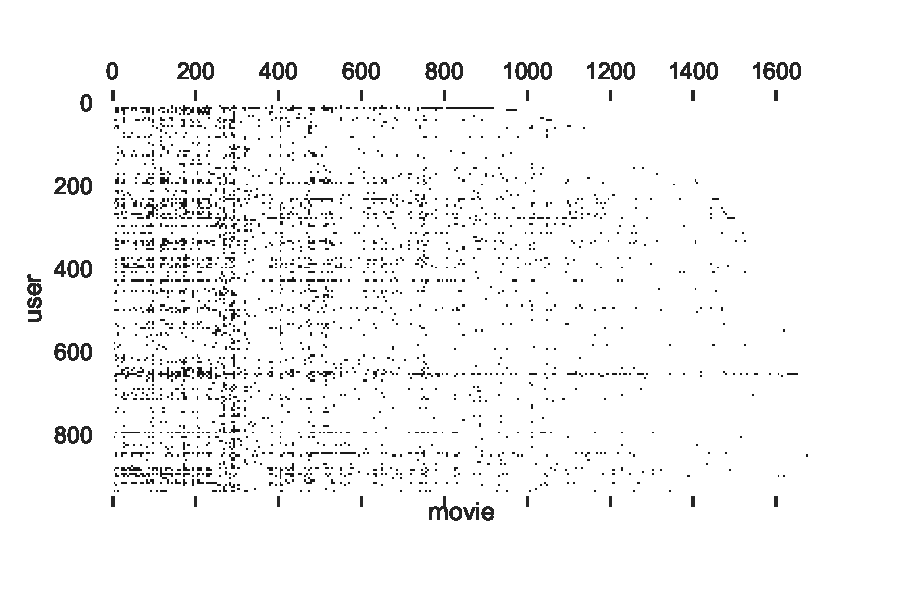
\includegraphics[scale=0.53]{./images/sparse.pdf}
  \caption{Representation of the sparsity of the $Y$ matrix.}
  \label{fig:sparse_fig}
\end{figure}

\end{frame}
%%%%%%%%%%%%%%%%%%%%%%%%%%%%%%%%%%%%%%%%%%%%%%%%%%%%%%%%%%%%%%%%%%%%%%%%%%%%%%%


%%%%%%%%%%%%%%%%%%%%%%%%%%%%%%%%%%%%%%%%%%%%%%%%%%%%%%%%%%%%%%%%%%%%%%%%%%%%%%%
\subsection{Size reduction}
\label{sec:reduction}
%%%%%%%%%%%%%%%%%%%%%%%%%%%%%%%%%%%%%%%%%%%%%%%%%%%%%%%%%%%%%%%%%%%%%%%%%%%%%%%

%%%%%%%%%%%%%%%%%%%%%%%%%%%%%%%%%%%%%%%%%%%%%%%%%%%%%%%%%%%%%%%%%%%%%%%%%%%%%%%
\begin{frame}{Size reduction}
\begin{onlyenv}<1>
\begin{itemize}
    \item decomposition of the $Y$ matrix, 
    \item product of two sub-matrix, 
    \item size reduction.
\end{itemize}
\end{onlyenv}
\begin{onlyenv}<2->
\begin{itemize}
    \item decomposition of the $Y$ matrix, 
    \item product of two sub-matrix, 
    \item size reduction.
\end{itemize}
    \begin{figure}[H]
\centering
  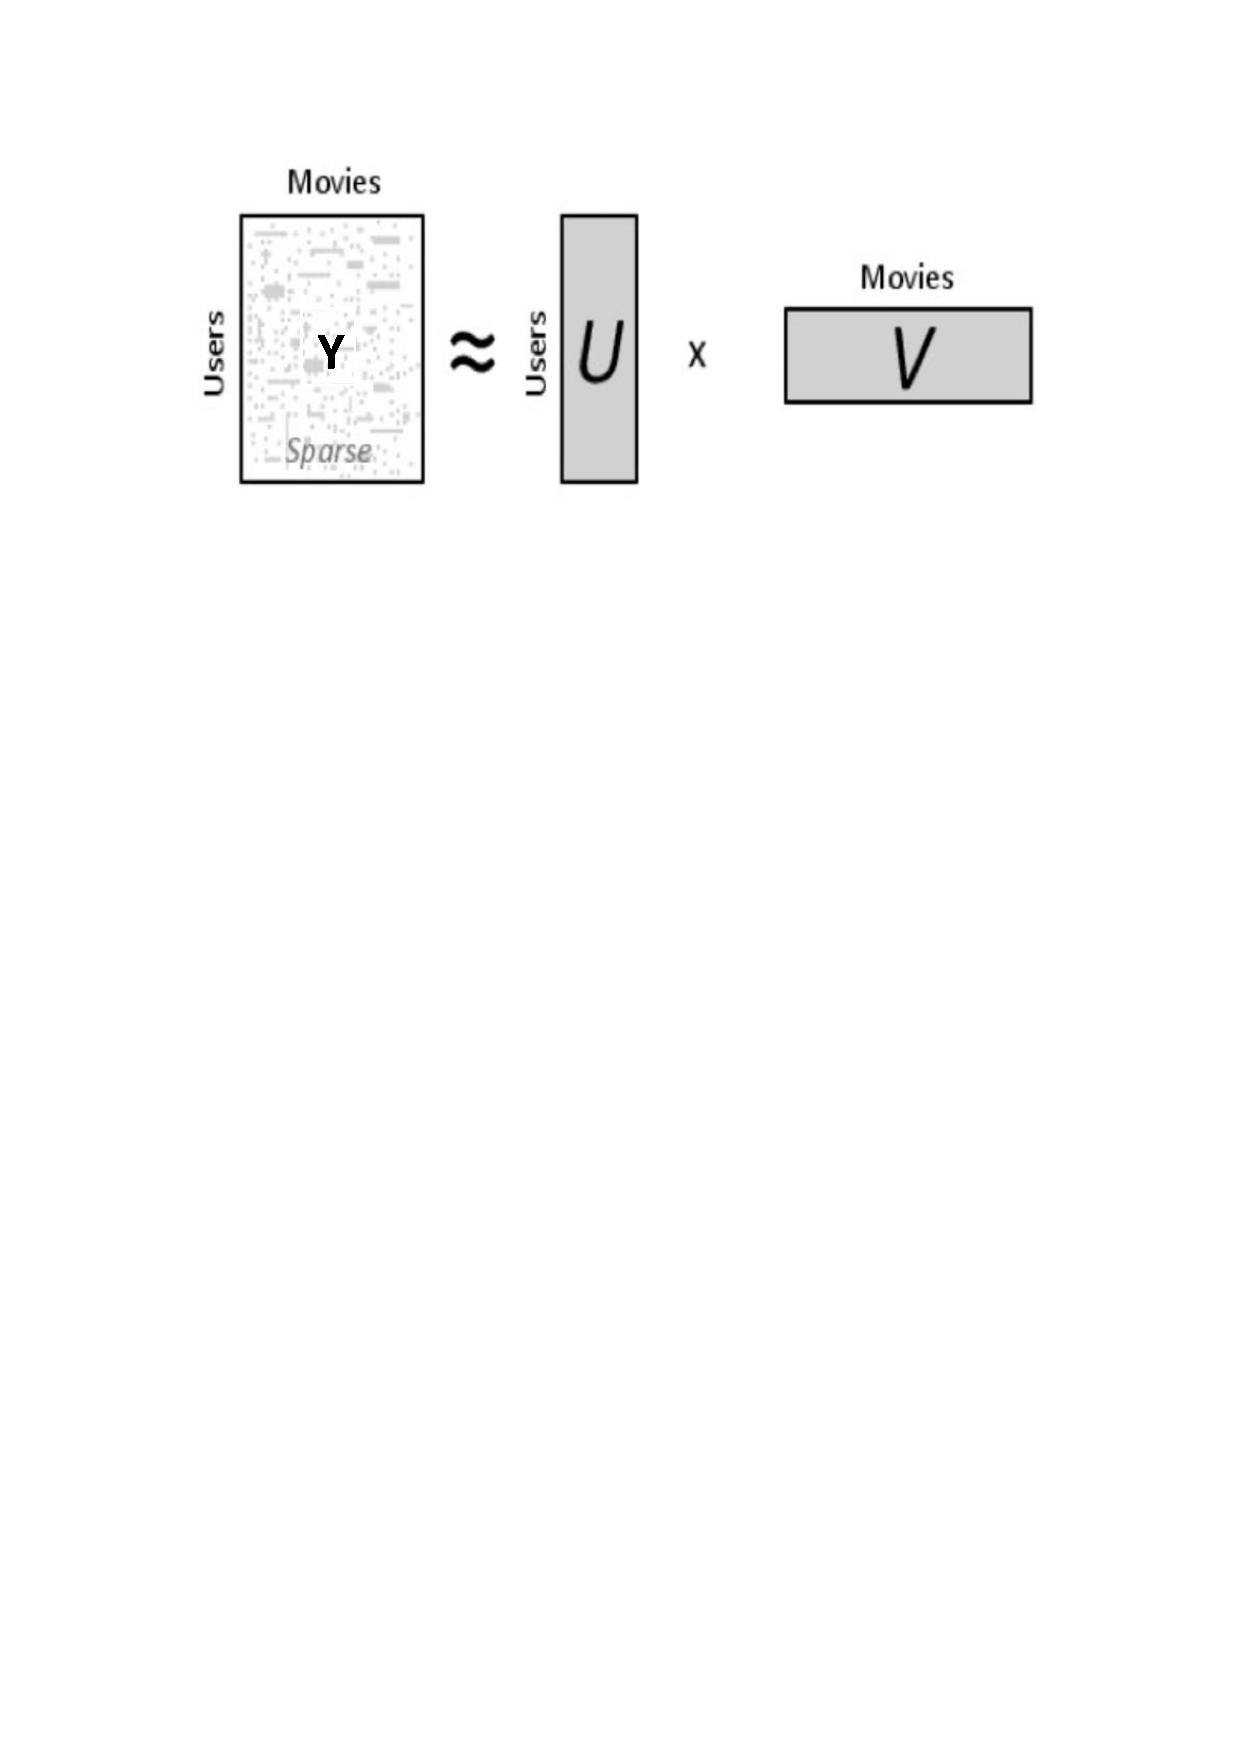
\includegraphics[scale=0.4]{./images/facto.pdf}
  \caption{$Y$-matrix factorisation.}
  \label{fig:facto}
\end{figure}
\end{onlyenv}
\end{frame}
%%%%%%%%%%%%%%%%%%%%%%%%%%%%%%%%%%%%%%%%%%%%%%%%%%%%%%%%%%%%%%%%%%%%%%%%%%%%%%%

%%%%%%%%%%%%%%%%%%%%%%%%%%%%%%%%%%%%%%%%%%%%%%%%%%%%%%%%%%%%%%%%%%%%%%%%%%%%%%%
\begin{frame}{Singular value decomposition}
  \begin{figure}[H]
\centering
  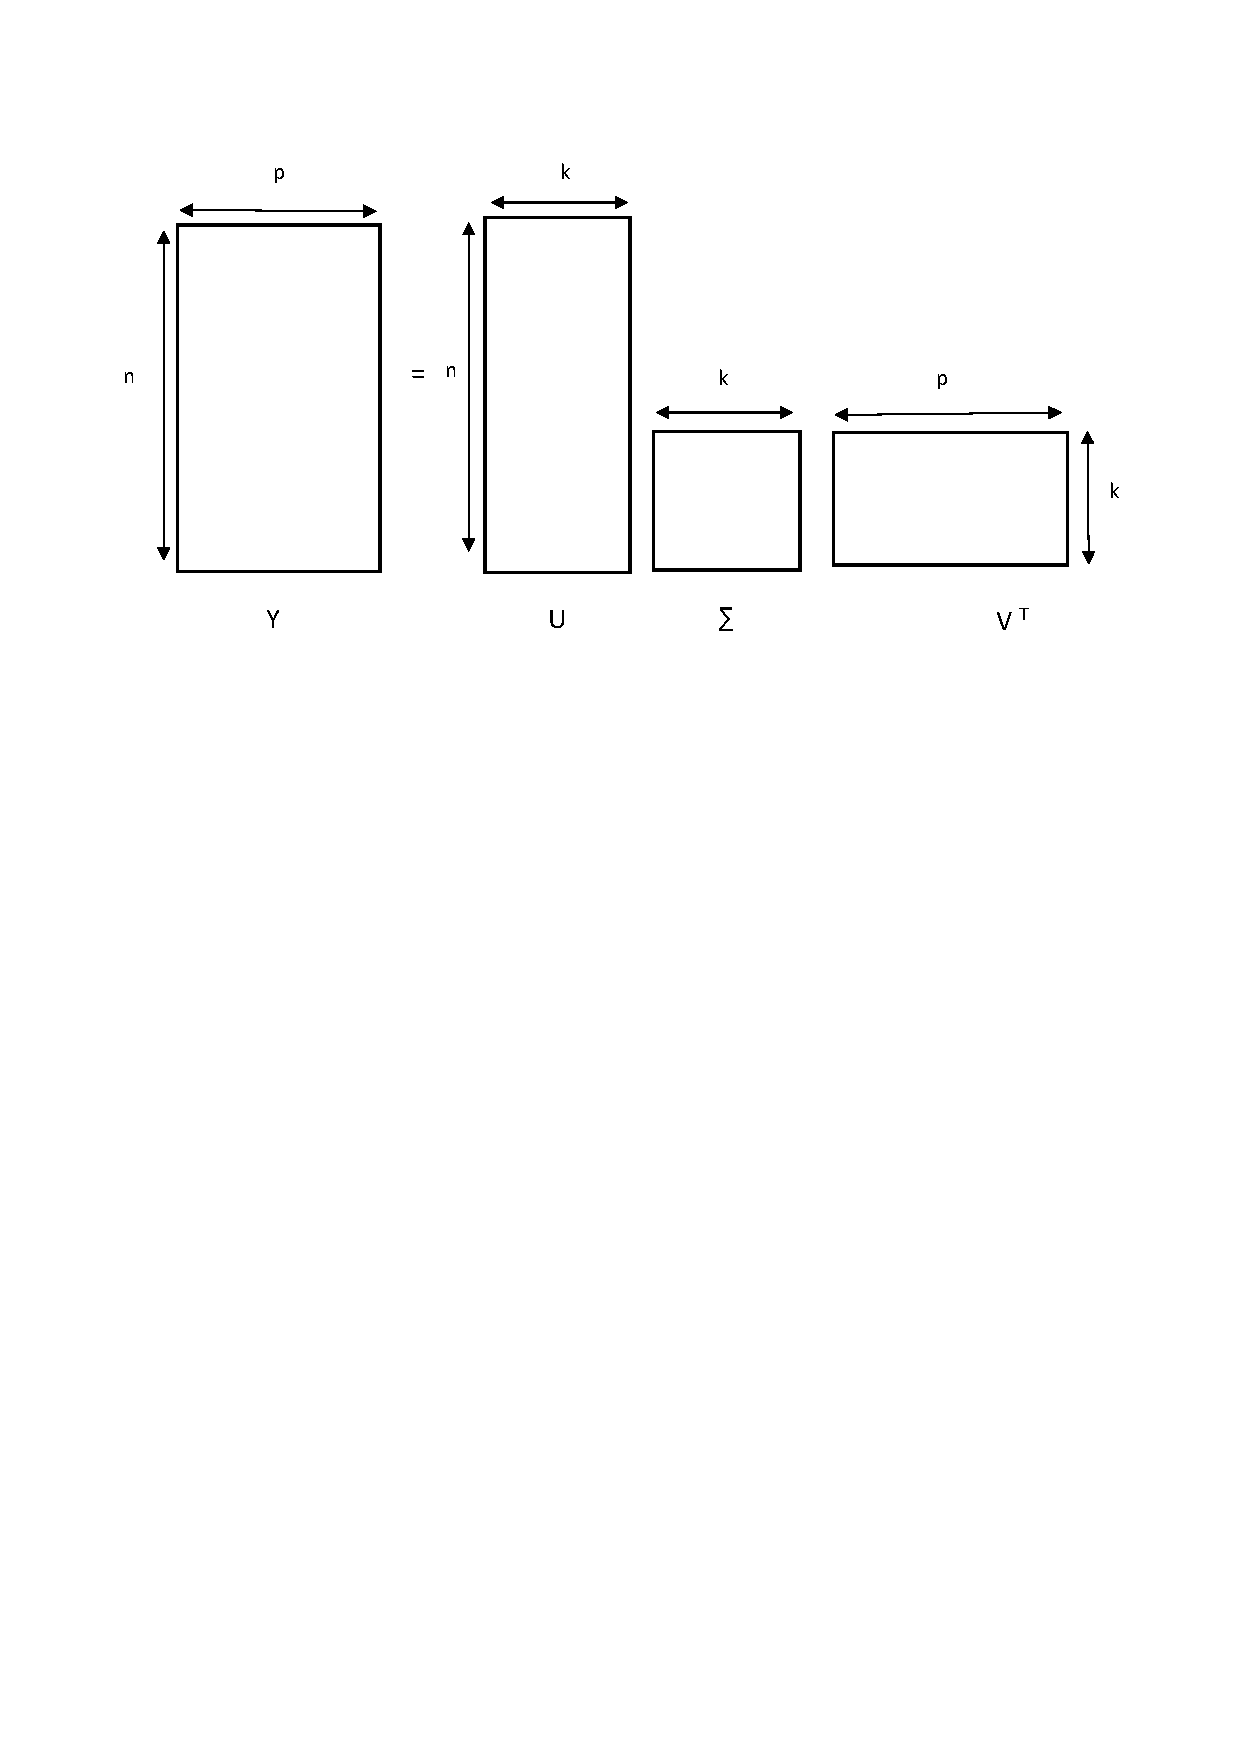
\includegraphics[scale=0.4]{./images/svd.pdf}
  \caption{Reduced SVD.}
  \label{fig:svd}
\end{figure} 
\begin{align*}
    \longrightarrow \text{ }& n=943,\\
    \longrightarrow \text{ }& p=1682,\\
    \longrightarrow \text{ }& k=6.
\end{align*}
\end{frame}
%%%%%%%%%%%%%%%%%%%%%%%%%%%%%%%%%%%%%%%%%%%%%%%%%%%%%%%%%%%%%%%%%%%%%%%%%%%%%%%

%%%%%%%%%%%%%%%%%%%%%%%%%%%%%%%%%%%%%%%%%%%%%%%%%%%%%%%%%%%%%%%%%%%%%%%%%%%%%%%
\begin{frame}{Loss function}
\begin{onlyenv}<1>
    Loss function used:
    $$L=\sum_{i,j \in DF} (y_{ij} - \hat{y}_{ij})^2 + \lambda\left(\sum_i || u_i ||^2 + \sum_j || v_j ||^2\right)$$
\end{onlyenv}
\begin{onlyenv}<2->
    Loss function used:
    $$L=\sum_{i,j \in DF} (y_{ij} - \hat{y}_{ij})^2 + \lambda\left(\sum_i || u_i ||^2 + \sum_j || v_j ||^2\right)$$
    where 
    \begin{itemize}
        \item $DF$ is the dataset, 
        \item $\hat{y}_{ij}$ corresponds to the prediction of the rating $y_{ij}$,
        \item quadratic objective function,
        \item minimize the difference between ratings in our dataset and predictions made.
    \end{itemize}
\end{onlyenv}
\end{frame}
%%%%%%%%%%%%%%%%%%%%%%%%%%%%%%%%%%%%%%%%%%%%%%%%%%%%%%%%%%%%%%%%%%%%%%%%%%%%%%%

%%%%%%%%%%%%%%%%%%%%%%%%%%%%%%%%%%%%%%%%%%%%%%%%%%%%%%%%%%%%%%%%%%%%%%%%%%%%%%%
%%%%%%%%%%%%%%%%%%%%%%%%%%%%%%%%%%%%%%%%%%%%%%%%%%%%%%%%%%%%%%%%%%%%%%%%%%%%%%%
\section{Conclusion}
%%%%%%%%%%%%%%%%%%%%%%%%%%%%%%%%%%%%%%%%%%%%%%%%%%%%%%%%%%%%%%%%%%%%%%%%%%%%%%%
%%%%%%%%%%%%%%%%%%%%%%%%%%%%%%%%%%%%%%%%%%%%%%%%%%%%%%%%%%%%%%%%%%%%%%%%%%%%%%%

%%%%%%%%%%%%%%%%%%%%%%%%%%%%%%%%%%%%%%%%%%%%%%%%%%%%%%%%%%%%%%%%%%%%%%%%%%%%%%%
\begin{frame}{Conclusion}
\begin{itemize}
    \item Lot of missing data, 
    \item predict the ratings that a user would give to a unseen movie,
    \item matrix factorisation to reduce dimension, 
    \item sparse matrix,
    \item reduced singular value decomposition.
\end{itemize}
\end{frame}
%%%%%%%%%%%%%%%%%%%%%%%%%%%%%%%%%%%%%%%%%%%%%%%%%%%%%%%%%%%%%%%%%%%%%%%%%%%%%%%

%%%%%%%%%%%%%%%%%%%%%%%%%%%%%%%%%%%%%%%%%%%%%%%%%%%%%%%%%%%%%%%%%%%%%%%%%%%%%%%
\begin{frame}{Bibliography}
\nocite{*}
\printbibliography
\end{frame}
%%%%%%%%%%%%%%%%%%%%%%%%%%%%%%%%%%%%%%%%%%%%%%%%%%%%%%%%%%%%%%%%%%%%%%%%%%%%%%

%%%%%%%%%%%%%%%%%%%%%%%%%%%%%%%%%%%%%%%%%%%%%%%%%%%%%%%%%%%%%%%%%%%%%%%%%%%%%%
\addtocounter{framenumber}{-1}
\begin{frame}[plain]{}
\begin{center}
    \LARGE\color{marron}
\textbf{Thank you!}
\end{center}
\end{frame}
%%%%%%%%%%%%%%%%%%%%%%%%%%%%%%%%%%%%%%%%%%%%%%%%%%%%%%%%%%%%%%%%%%%%%%%%%%%%%%
\end{document}